\section{\label{sec:SoA}Introduction}
Developing products, especially lightweight structures, 
requires variety of steps to come from the original idea to the final product.
One approach to follow these steps to result in a successful production 
are described in the guidelines of VDI 2206 \cite{gausmeier2002} and VDI 2221 \cite{Jansch2006THEDO}.
These guidelines give a general methodology for designing technical systems and products, 
by introducing a methodical and systematic designing procedure, to work with maximum efficiency.
Since the first introduction in 1993 these guidelines have been applied within mechanical engineering, precision mechanics, 
switches and software development and the planning of process engineering \cite{pahl_beitz_2013}. 
Depending on the individual outcome steps might be repeated in as part of cyclic quality enforcing technique.
Especially in lightweight design the analysis, design and manufacturing processes are so strong connected, 
that they all have to be considered in every phase of the development process (fig. \ref{pic:interactive-design}).
The amount of cyclic repeats do increase with higher demands on the products efficiency and error margin.
These causes it to be one of the main factors for increased development time and 
also reduces the amount of reusable components with slightly changes in the product demand.\\
\begin{figure}[h]
    \centering
    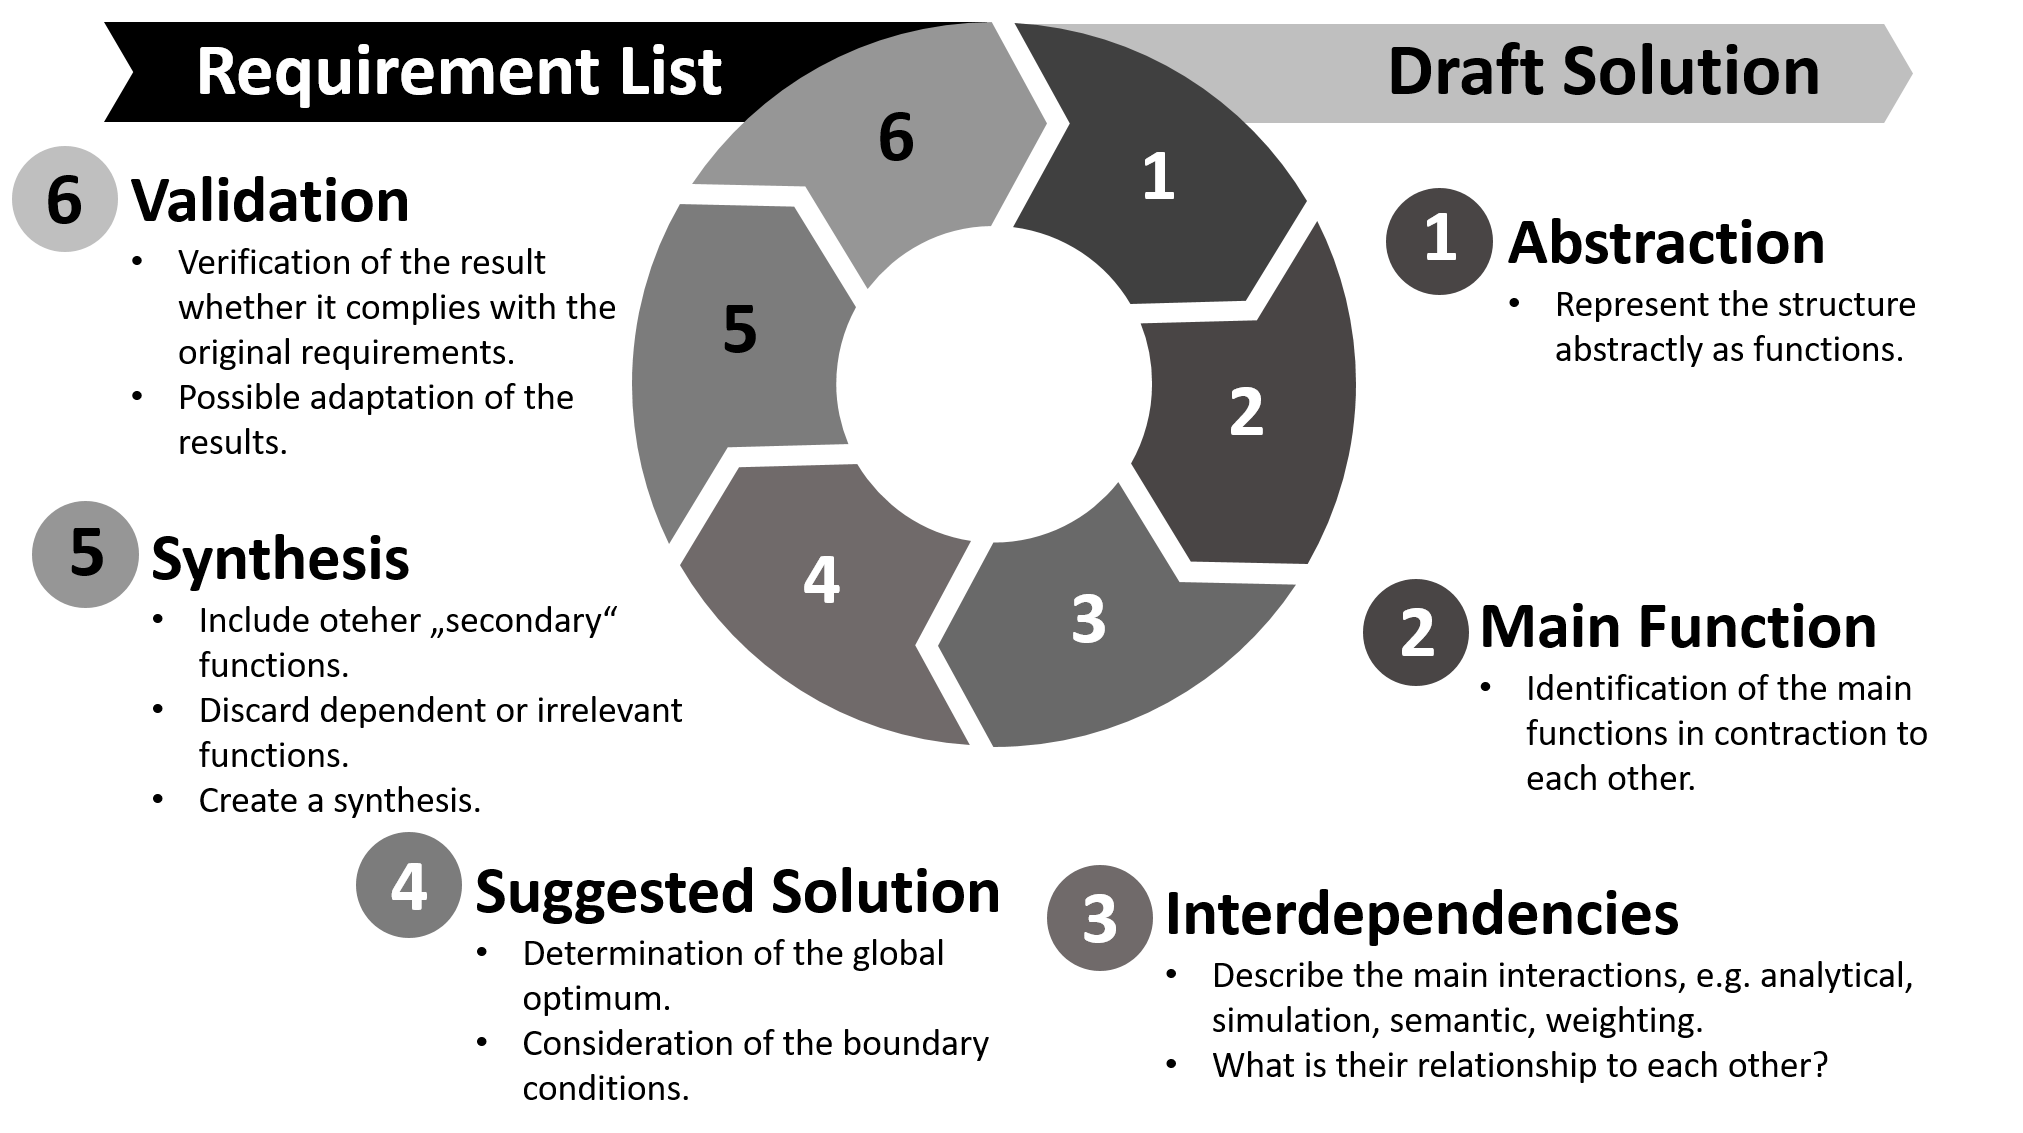
\includegraphics[scale=0.4]{pics/cyclic-design.PNG}
    \caption{\label{pic:interactive-design} "A spiral development approach for complex function‐integrative systems." \cite{Modler2020}}
\end{figure}\\
Even before the rise of digital twins \cite{Leitenberger2021} solution have been applied to digital represnet each functionality and each dependencies of asystem.
Starting in 1970, E. Allen layed the fundament of current resarch with his work on directed graphs \cite{allen_control_1970}.
Today solutions like ANSYS, SiemensNX, CAMUNDA, etc. implement workflow engines to automate processes which are presented as directed graphes \cite{noauthor_dynamo_2020, noauthor_function_2020, noauthor_systems_2020}.
These engines are build on certain requirements, like automating some of the simulation work and safing time by reusing models.
But are limited in the kind of systems they can represents.\\
One reasons is that only linear graphs, with a few exceptions are represented and solved.
ANSYS for example, bey default only allows linear graphs, with the only excepts, being parameter studies.
While this is often is enough, its a big issue if interdependencies behave non-linear, like the dependencies in structural batteries, 
where structural and electrical properties are strongly intertwined \cite{Asp2021}.
On the other side problems is that general non-linear graph representations have been proofen to be Turing-complete.
Therefore it is impossible to find an algorithm that finds a converged solution to all systems \cite{Ajtai1990}.\\
Further the use is often limited on to a certain system or software ecosystem.
This is mostly, due to a lack of standardization in model representations.
But there is one exception: for the planning, designing, construction and mantaining of builds the 
"Building information modeling" (BIM) has been developed since the 1970s and is an international agreed standard with the ISO 19650 since 2019.
While standards for the problem of designing problems a international standard is still missing, some notable efforts have been made \cite{noauthor_modelica_nodate, mukherjee_hierarchical_1999,  Berschik2021}.
With system implementing its own standards, the number of different data formats increases.
Further increasing the complexity of modelling multi-disciplinary systems.
\begin{figure}[h]
    \centering
    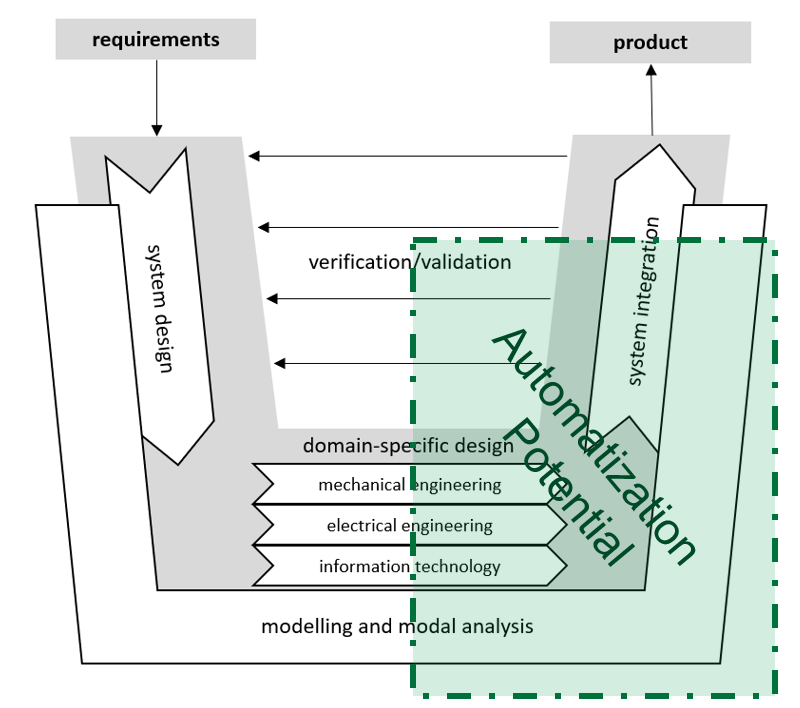
\includegraphics[scale=0.6]{pics/VDI_2206.PNG}
    \caption{\label{pic:VDI2206} Automatisation potential in the VDI 2206 Guidline \cite{Jansch2006THEDO}.}
\end{figure}\\
Another issue which can arise in design processes is the amount of optimization work, which takes a major part of the development time in high effient products.
Optimizations therefor stretches, from topologie optimization, to varaints comparision and parameter tuning \cite{hornby_automated_2006, khalafallah_electimize_2011, evans_aerodynamic_2017, slagter_perform_2020}. 
This lead to an extra major potential for time saving in lightweight design, as shown in figure \ref{pic:VDI2206}.\\
Assuming that the complex multi-disciplinary systems can be modelled sufficiently, the question of how to find the optimal solution rises.
Therfore algorithm has been developed, which requires up to none system knowledge.
Algorithm like simulated annealing \cite{khachaturyan_thermodynamic_1981}, 
evolutionary algorithm \cite{wu_ensemble_2019}, particle swarm optimization \cite{Kennedy1995} and Bayesian optimization \cite{marcuk_optimization_1975}
are the most popular ones, by have proofen to find find the global optimum and not to fall in local minima.\\
Following the state of the art, this paper wants to introduce it an open-source information based workflow engine for design processes.
The proposed work will therfore fokus on the representation of complex multi-domain tasks and implements optimization techniques to find the best product for a custom use case.